\documentclass[letterpaper,10pt]{article}
\usepackage[top=2cm, bottom=1.5cm, left=1cm, right=1cm]{geometry}
\usepackage{amsmath, amssymb, amsthm, graphicx}
\usepackage{fancyhdr}
\pagestyle{fancy}

\lhead{\today}
\chead{MATH498- Spatial Processes in Biology}
\rhead{Justin Hood}

\newcommand{\Z}{\mathbb{Z}}
\newcommand{\Q}{\mathbb{Q}}

\begin{document}
\begin{description}
\item[1.]\hfill \\
We consider the table of molecular weights and diffusion coefficients. Our rule of thumb for computing D from M is $D\approx M^{-1/3}$. Plotting the table on a log-log plot yields the result below.
\begin{center}
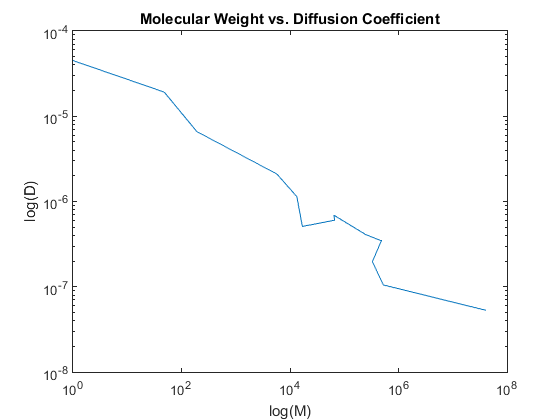
\includegraphics{pureplot.png}
\end{center}
We note that the plot is linear with values decreasing as M increases, as expected. Given that we can assume the data is proportional by the rule of thumb, we consider a line of best fit to be of the form,
\[D=beta_1M^{-\frac{1}{3}}+\beta_2\]
Using a linear fitting method, I determined the coefficients to be,
\begin{align*}
\beta_1 &\approx 4.779\times 10^{-5}\\
\beta_2 &\approx 1.399\times 10^{-7}
\end{align*}
Plotting the resultant line over the data yields the following result; which, from a purely visual inspection seems to support the rule of thumb as being accurate.
\begin{center}
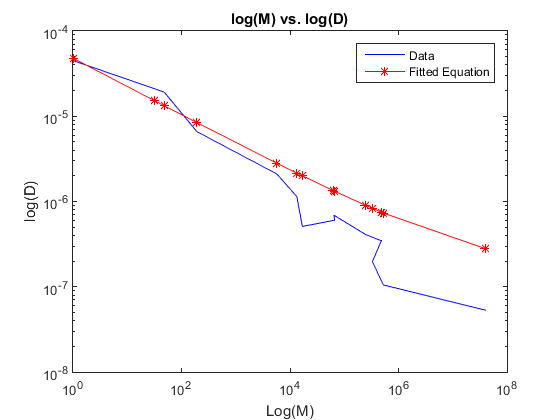
\includegraphics{bestfit.png}
\end{center}
\end{description}


\end{document}
